\begin{grafico}[H]
    \centering
    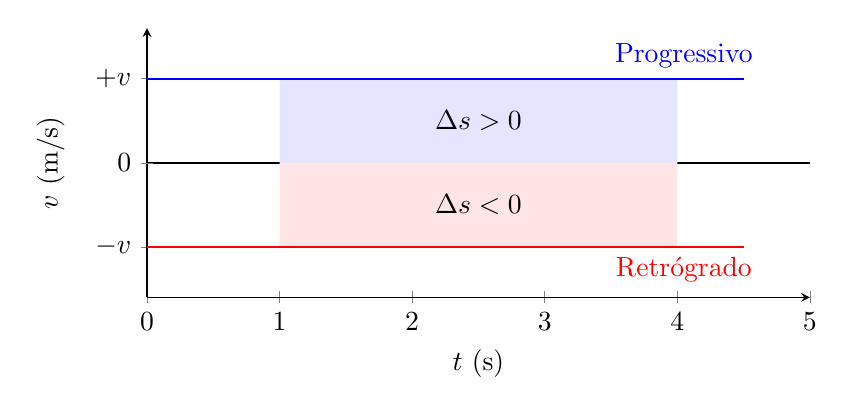
\begin{tikzpicture}
    \begin{axis}[
        axis lines = left,
        xlabel = {$t$ (s)},
        ylabel = {$v$ (m/s)},
        width=10cm, height=5cm,
        xmin=0, xmax=5,
        ymin=-8, ymax=8,
        extra y ticks={0},
        extra y tick style={grid=major, grid style={black, thick}},
        ytick={-5, 5},
        yticklabels={$-v$, $+v$}
    ]
    % Área e linha para velocidade positiva
    \addplot [fill=blue!10, draw=none, domain=1:4] {5} \closedcycle;
    \addplot [domain=0:4.5, thick, blue] {5} node[pos=0.9, above] {Progressivo};
    
    % Área e linha para velocidade negativa
    \addplot [fill=red!10, draw=none, domain=1:4] {-5} \closedcycle;
    \addplot [domain=0:4.5, thick, red] {-5} node[pos=0.9, below] {Retrógrado};
    
    \node at (axis cs: 2.5, 2.5) {$\Delta s > 0$};
    \node at (axis cs: 2.5, -2.5) {$\Delta s < 0$};
    \end{axis}
    \end{tikzpicture}
    \caption{Gráfico de velocidade no MRU. A área sombreada representa o deslocamento $\Delta s = v \cdot \Delta t$.}
\end{grafico}